\chapter{Sound: Production and Propagation}\label{ch:g7:sound-production}

You have known since childhood that \omterm{def:g3:sound-around-us:sound}{sound} is born in a trembling
and dies in emptiness --- the rice grains danced, the bell in the
jar fell silent. What you lacked was the messenger's name. Now
you own the molecular world, and \omterm{def:g3:sound-around-us:sound}{sound}'s whole journey --- from
a guitar string to your eardrum, through \omterm{def:g2:air-around-us:air}{air}, water or steel ---
can finally be watched from inside.

\section{The messengers}

\begin{definition}[Medium]\label{def:g7:sound-production:medium}
A \emph{medium}\index{medium} (plural \emph{media}) is the
substance a \omterm{def:g3:sound-around-us:sound}{sound} travels through: \omterm{def:g2:air-around-us:air}{air}, water, wood, steel ---
any state will serve, for all are crowds of \omterm{def:g7:states-of-matter:molecule}{molecules}. What no
\omterm{def:g3:sound-around-us:sound}{sound} can cross is the absence of a crowd: vacuum, the empty
stage.
\end{definition}

\begin{proposition}[How sound travels]\label{prop:g7:sound-production:travel}
A vibrating source shoves the \omterm{def:g7:states-of-matter:molecule}{molecules} beside it; they crowd
against their neighbors and rebound; the neighbors shove the
next rank in turn. The shove --- a traveling squeeze of the
crowd --- races outward from the source in every direction,
\omterm{def:g7:states-of-matter:molecule}{molecule} relaying \omterm{def:g7:states-of-matter:molecule}{molecule}, though each \omterm{def:g7:states-of-matter:molecule}{molecule} itself only
jiggles about its place. \omterm{def:g3:sound-around-us:sound}{Sound} is the \emph{relay}, not the
runners: the message travels; the messengers stay home.
\end{proposition}

\begin{omfigure}
\begin{tikzpicture}[scale=0.85]
  \draw[thick] (0.2,0.4) -- (0.2,2.2);
  \draw[thick] (0.5,0.4) -- (0.5,2.2);
  \node[above, font=\small] at (0.35,2.3) {vibrating plate};
  \foreach \x in {1.0,1.25,1.5,2.4,3.3,4.2,4.45,4.7,5.6,6.5,
      7.4,7.65,7.9,8.8,9.7} {
    \fill[omDef] (\x,1.3) circle (0.11);
  }
  \draw[-Stealth, very thick, omThm] (1.0,2.0) -- (2.6,2.0);
  \node[above, font=\small, omThm] at (1.8,2.1)
    {the squeeze travels};
  \node[below, font=\small] at (1.3,0.8) {crowded};
  \node[below, font=\small] at (3.3,0.8) {spread};
  \node[below, font=\small] at (4.6,0.8) {crowded};
  \node[below, font=\small] at (6.5,0.8) {spread};
  \node[below, font=\small] at (7.8,0.8) {crowded};
\end{tikzpicture}

{\small \omterm{def:g3:sound-around-us:sound}{Sound} inside the \omterm{def:g2:air-around-us:air}{air}: the source's shove travels as a
relay of squeezes through the molecular crowd --- each \omterm{def:g7:states-of-matter:molecule}{molecule}
jiggling in place, the pattern racing on.}
\end{omfigure}

\begin{example}[The jar, explained at last]\label{ex:g7:sound-production:jar}
The famous silenced bell now confesses its mechanism. Pumping
out the \omterm{def:g2:air-around-us:air}{air} removes the crowd: the bell's trembling walls shove
at nothing, no relay forms, and no message crosses the glass.
The bell never stopped --- it lost its messengers. And space's
great silence follows at once: between the \omterm{def:g4:solar-system:star}{stars} there is no
crowd to carry a cry.
\end{example}

\begin{example}[Loud, quiet, and worn out]\label{ex:g7:sound-production:loud}
A harder shove makes a stronger squeeze: louder \omterm{def:g3:sound-around-us:sound}{sound}. And as
the relay spreads --- pond-rings in three dimensions --- each
squeeze is shared over a vaster and vaster shell of crowd,
weakening with distance: why shouts fade, and why the
neighbor's music is a murmur through two walls. Nothing of this
needed new laws: crowd physics pays for everything.
\end{example}

\begin{omfigure}
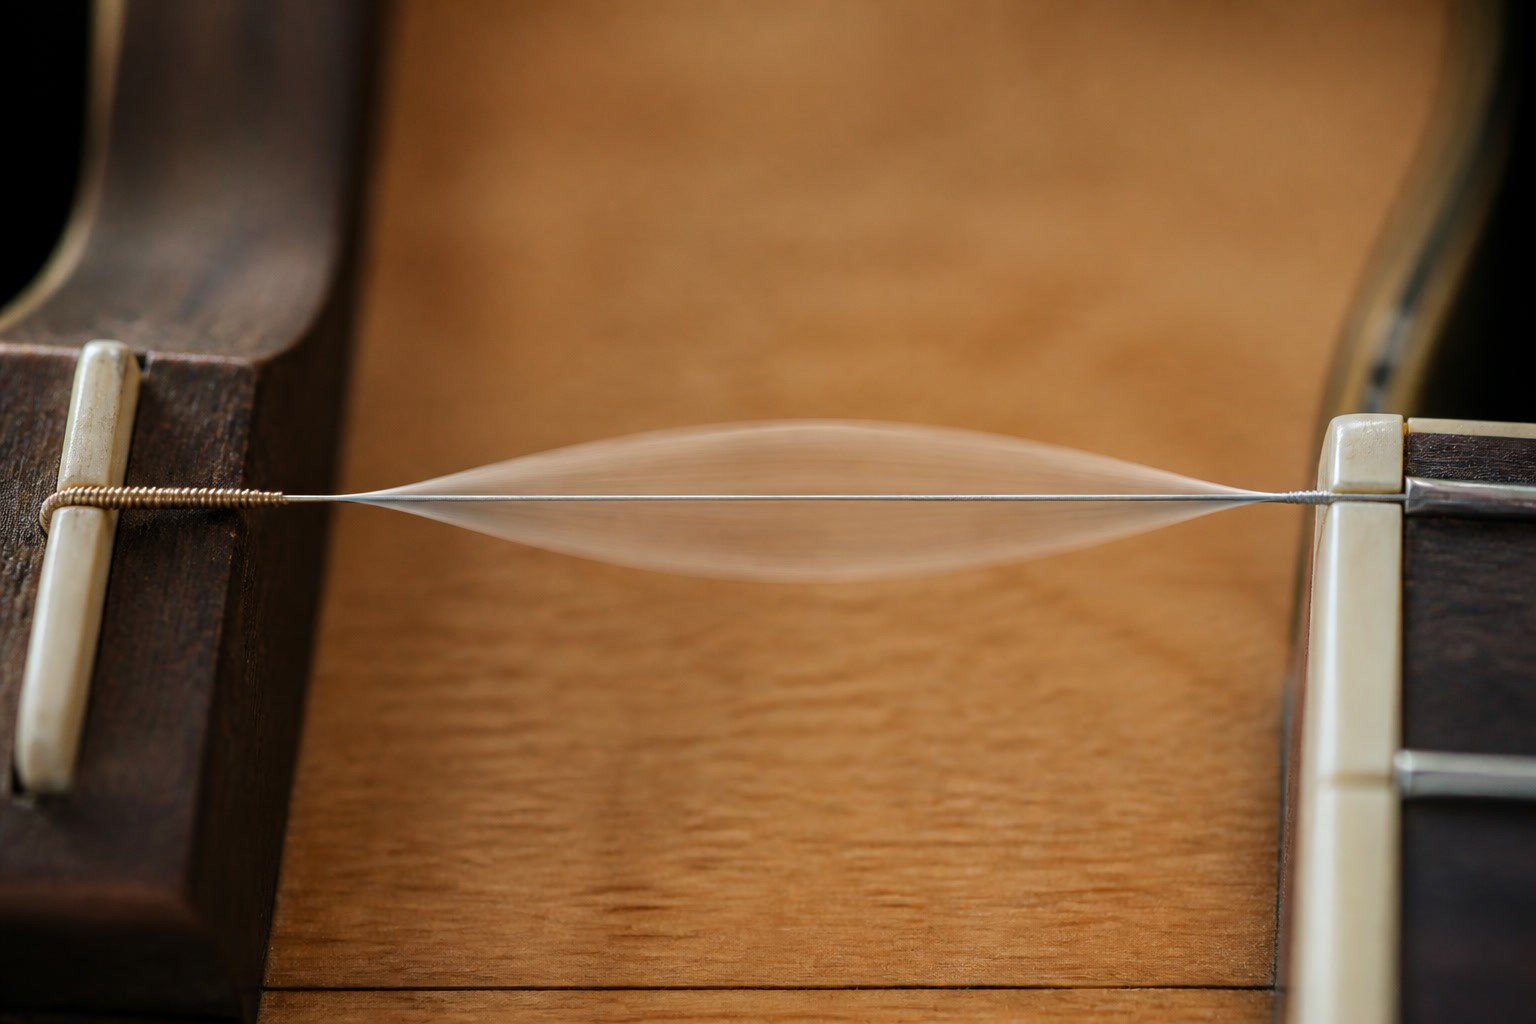
\includegraphics[width=0.55\linewidth]{images/book1/ai/g7-sound-string-blur.jpg}

{\small A plucked string photographed mid-song: the \omterm{def:g3:sound-around-us:vibration}{vibration} blurs it into a wide band, widest at the middle, still at its two fixed ends.}
\end{omfigure}

\section{Every medium has its pace}

\begin{proposition}[The speed of sound depends on the medium]\label{prop:g7:sound-production:speeds}
The relay's \omterm{def:g7:motion-average-speed:formula}{speed} is a property of the crowd:
\begin{enumerate}
  \item in \omterm{def:g2:air-around-us:air}{air}: about \qty{340}{m/s};
  \item in water: about \qty{1500}{m/s} --- four times faster;
  \item in steel: about \qty{5000}{m/s} --- fifteen times
        faster than \omterm{def:g2:air-around-us:air}{air}.
\end{enumerate}
The pattern: the more tightly a \omterm{def:g7:sound-production:medium}{medium}'s \omterm{def:g7:states-of-matter:molecule}{molecules} touch, the
faster they hand the shove along. Flying \omterm{def:g2:air-around-us:air}{air} \omterm{def:g7:states-of-matter:molecule}{molecules} must
first cross gaps to deliver; water's touching crowd relays
briskly; steel's locked ranks pass the message almost
hand-to-hand.
\end{proposition}

\begin{omfigure}
\begin{tikzpicture}
\begin{axis}[omaxis, width=10.4cm, height=4.6cm, xbar,
    xlabel={speed of sound (\unit{m/s})},
    symbolic y coords={air, water, steel},
    ytick=data, xmin=0, xmax=5600,
    bar width=9pt, xtick={340,1500,5000},
    every axis plot/.append style={fill=omDef, fill opacity=0.55,
      draw=omDef}]
  \addplot coordinates {(340,air) (1500,water) (5000,steel)};
\end{axis}
\end{tikzpicture}

{\small Three crowds, three paces: the tighter the \omterm{def:g7:states-of-matter:molecule}{molecules}'
contact, the faster the relay.}
\end{omfigure}

\begin{example}[Old scenes, new numbers]\label{ex:g7:sound-production:scenes}
The scout's ear on the rail: the steel relay outruns the \omterm{def:g2:air-around-us:air}{air}'s
by a factor of fifteen --- the rail's warning arrives long
before the rumble. Whales' songs crossing seas: water's swift,
generous relay. And your own voice \omterm{def:g3:sound-around-us:sound}{sounds} strange on recordings
partly because, speaking, you hear yourself through the skull's
bone-relay as well as through \omterm{def:g2:air-around-us:air}{air} --- two media, two versions,
and only other people ever hear the air-only one.
\end{example}

\section{Sound with a stopwatch}

\begin{method}[Measuring the speed of sound]\label{met:g7:sound-production:measure}
The oldest method still works on any sports field:
\begin{enumerate}
  \item a partner stands a measured \qty{680}{m} away (two
        field-lengths and a bit --- pace it or use the field's
        markings) with two pan lids;
  \item they clash the lids overhead: you \emph{see} the strike
        instantly (\omterm{def:g1:light-and-shadows:source}{light}'s trip is as good as instant), and
        start the stopwatch on the flash of motion;
  \item stop on the arriving clang: expect very nearly
        \qty{2}{s};
  \item compute: $v = d/t = 680 \div 2 = \qty{340}{m/s}$.
\end{enumerate}
Repeat and average --- reaction times scatter, as the honest
measurement chapter taught. Thunder-counting is this method run
backward: knowing $v$, the silent seconds hand you the
distance.
\end{method}

\begin{example}[The echo, computed]\label{ex:g7:sound-production:echo}
A clap toward a cliff returns in \qty{3}{s}. The \omterm{def:g3:sound-around-us:sound}{sound} traveled
to the cliff and back: $d_{\text{round trip}} = 340 \times 3 =
\qty{1020}{m}$, so the cliff stands at half: \qty{510}{m}. The
rule of every \omterm{ex:g4:how-sound-travels:echo}{echo} sum: the measured time pays for the round
trip --- forgetting the ``and back'' is the classic slip, and
doubles every answer wrongly.
\end{example}

\begin{example}[Sonar, in earnest]\label{ex:g7:sound-production:sonar}
The survey ship's sonar clicks downward; the seabed's \omterm{ex:g4:how-sound-travels:echo}{echo}
returns in \qty{0.6}{s}. In \emph{water}, $d = 1500 \times 0.6 =
\qty{900}{m}$ round trip: depth \qty{450}{m}. Dolphins and bats
run the same arithmetic by instinct; ships print it on charts.
Note the discipline: the \omterm{def:g7:sound-production:medium}{medium} chooses the \omterm{def:g7:motion-average-speed:formula}{speed} --- feeding an
underwater \omterm{ex:g4:how-sound-travels:echo}{echo} the \omterm{def:g2:air-around-us:air}{air}'s $340$ is the chapter's second classic
slip.
\end{example}

\begin{remark}[What ``fast'' still is not]\label{rem:g7:sound-production:light}
Steel's \qty{5000}{m/s} \omterm{def:g3:sound-around-us:sound}{sounds} heroic --- until \omterm{def:g1:light-and-shadows:source}{light} is
recalled. In the storm, the flash's trip counts as instant while
thunder jogs its kilometre in three seconds; and no \omterm{def:g7:sound-production:medium}{medium}, not
steel, not diamond, brings \omterm{def:g3:sound-around-us:sound}{sound} within shouting distance of
\omterm{def:g1:light-and-shadows:source}{light}'s pace. Exactly how fast \omterm{def:g1:light-and-shadows:source}{light} runs --- and how humans
finally clocked something that crosses a room in a
hundred-millionth of a second --- is next year's story, with a
chapter of its own.
\end{remark}

\section{Exercises}

\begin{exercise}[$\star$]\label{exo:g7:sound-production:1}
What is a \omterm{def:g7:sound-production:medium}{medium}? Name three, and the one ``\omterm{def:g7:sound-production:medium}{non-medium}'' no
\omterm{def:g3:sound-around-us:sound}{sound} can cross.
\end{exercise}

\begin{exercise}[$\star$]\label{exo:g7:sound-production:2}
In the relay picture, what travels from source to ear --- and
what does each individual \omterm{def:g7:states-of-matter:molecule}{molecule} do?
\end{exercise}

\begin{exercise}[$\star$]\label{exo:g7:sound-production:3}
Explain the silenced bell-in-the-jar with \omterm{def:g7:states-of-matter:molecule}{molecules} --- and why
films' roaring space battles are physics fiction.
\end{exercise}

\begin{exercise}[$\star$]\label{exo:g7:sound-production:4}
Give the three \omterm{def:g7:motion-average-speed:formula}{speeds} of the chapter's table, and the pattern
connecting a \omterm{def:g7:sound-production:medium}{medium}'s molecular arrangement to its pace.
\end{exercise}

\begin{exercise}[$\star$]\label{exo:g7:sound-production:5}
Why does the scout's rail-message outrun the \omterm{def:g2:air-around-us:air}{air}'s? By roughly
what factor?
\end{exercise}

\begin{exercise}[$\star$]\label{exo:g7:sound-production:6}
In the field measurement, why is watching the lids' strike as
good as a starting gun at the source itself?
\end{exercise}

\begin{exercise}[$\star$]\label{exo:g7:sound-production:7}
A clap's \omterm{ex:g4:how-sound-travels:echo}{echo} from a warehouse wall returns in \qty{1}{s}. How
far is the wall? Name the slip that would answer
\qty{340}{m}.
\end{exercise}

\begin{exercise}[$\star$]\label{exo:g7:sound-production:8}
A ship's sonar \omterm{ex:g4:how-sound-travels:echo}{echo} returns in \qty{2}{s}. The depth? Name the
slip that would use \qty{340}{m/s}.
\end{exercise}

\begin{exercise}[$\star\star$]\label{exo:g7:sound-production:9}
Fireworks over the bay: you see the burst, and hear it
\qty{2.5}{s} later. How far is the shell? Why is the same
computation useless for judging the distance of a \emph{jet}
you can hear but not see?
\end{exercise}

\begin{exercise}[$\star\star$]\label{exo:g7:sound-production:10}
A swimmer with one ear underwater hears the pool's underwater
speaker before a friend on the deck hears it through \omterm{def:g2:air-around-us:air}{air} ---
though the friend stands nearer. Reconcile with the table.
\end{exercise}

\begin{exercise}[$\star\star$]\label{exo:g7:sound-production:11}
Old railway lore: put your ear to the rail and you hear the
train \emph{twice}. Explain the two arrivals, and compute the
gap for a train \qty{3}{km} away (steel at \qty{5000}{m/s},
\omterm{def:g2:air-around-us:air}{air} at \qty{340}{m/s} --- one decimal is enough).
\end{exercise}

\begin{exercise}[$\star\star\star$]\label{exo:g7:sound-production:12}
Design a measurement of the \omterm{def:g7:motion-average-speed:formula}{speed} of \omterm{def:g3:sound-around-us:sound}{sound} \emph{in water} for
a calm lake, using a waterproof clacker, a hydrophone (an
underwater microphone) \qty{750}{m} away, and a recorder that
also captures the clacker's airborne clap through a normal
microphone beside it. Explain how comparing the two recorded
arrival times yields water's \omterm{def:g7:motion-average-speed:formula}{speed} --- and compute the expected
gap between the two arrivals.
\end{exercise}

\section{Problem: The Canyon Survey}

\begin{problem}[{Weekend problem --- mapping the silent canyon
by ear; echoes, rails and river depths; the surveyor's
toolkit}]\label{pb:g7:sound-production:1}
A survey team maps a remote canyon with stopwatches, one sonar
\omterm{def:g6:measurement-in-science:measuring}{unit}, and the physics of this chapter. \omterm{def:g7:motion-average-speed:formula}{Speeds}: \omterm{def:g2:air-around-us:air}{air}
\qty{340}{m/s}, water \qty{1500}{m/s}, steel \qty{5000}{m/s}.

\medskip\noindent\textbf{Part I --- Widths by \omterm{ex:g4:how-sound-travels:echo}{echo}.}
\begin{enumerate}
  \item From the eastern rim, a clap's \omterm{ex:g4:how-sound-travels:echo}{echo} off the western
        wall returns in \qty{4}{s}. How wide is the canyon
        here?
  \item At a narrower point, the \omterm{ex:g4:how-sound-travels:echo}{echo} returns in \qty{1.5}{s}.
        The width?
  \item A surveyor standing \emph{between} two parallel walls
        claps once and hears two distinct \omterm{ex:g4:how-sound-travels:echo}{echoes}: after
        \qty{1}{s} and after \qty{2}{s}. How far is each wall,
        and how wide is the canyon on this line?
  \item Why does the biggest measurement error in Part I come
        from the stopwatch hand, not the formula? (Cite the
        wisdom of the repeated-measurement rule.)
\end{enumerate}

\medskip\noindent\textbf{Part II --- The river below.}
\begin{enumerate}[resume]
  \item The sonar \omterm{def:g6:measurement-in-science:measuring}{unit}, floated on the river, pings the bottom:
        \omterm{ex:g4:how-sound-travels:echo}{echo} in \qty{0.2}{s}. The river's depth?
  \item The same \omterm{def:g6:measurement-in-science:measuring}{unit} pinged sideways toward a submerged
        boulder returns an \omterm{ex:g4:how-sound-travels:echo}{echo} in \qty{0.4}{s}. Distance to
        the boulder?
  \item A teammate suggests saving batteries: ``shout from the
        boat and time the bottom \omterm{ex:g4:how-sound-travels:echo}{echo} by ear.'' Two physical
        reasons this fails where the sonar succeeds. (Think of
        the border between media, and of what a shout's \omterm{def:g2:air-around-us:air}{air}
        relay must do at the surface.)
  \item The riverbed drops sharply mid-channel: predict what
        the sonar's \omterm{ex:g4:how-sound-travels:echo}{echo} time does as the boat drifts across
        the drop.
\end{enumerate}

\medskip\noindent\textbf{Part III --- The old mining rail.}
A straight abandoned rail runs \qty{2}{km} along the canyon
floor to the mine gate.
\begin{enumerate}[resume]
  \item A hammer blow on the rail at the gate: compute the two
        arrival times at the surveyors' end --- through steel,
        and through \omterm{def:g2:air-around-us:air}{air}.
  \item The team hears rail-clang and air-boom separated by
        that gap. Explain how the \emph{gap alone} could
        \omterm{def:g6:measurement-in-science:measuring}{measure} the distance to the gate if the \qty{2}{km}
        were unknown (describe the reasoning; the computation
        is Part III's gift to the keen).
  \item Fog fills the canyon overnight --- useless for lamps
        and \omterm{def:g5:mirrors-reflection:reflection}{mirrors}. Which of the team's three measuring
        channels (\omterm{def:g3:sound-around-us:sound}{air-sound}, \omterm{def:g3:sound-around-us:sound}{water-sound}, \omterm{def:g3:sound-around-us:sound}{rail-sound}) does fog
        disturb least, and why?
  \item Write the surveyor's log: three sentences --- the
        round-trip rule, the medium-chooses-the-speed rule,
        and which single instrument (eye or ear) started every
        timing in the canyon, and why it may be trusted as
        ``instant''.
\end{enumerate}
\end{problem}
